\chapter{Research}
\label{ch:research}

For the project to be successful, research needs to be done on a range of topics including most notably RISC-V, as-well as other considered architectures, implementation languages and existing solutions. These are all discussed in the following sections.

\section{Architecture}
The project itself could of been produced for any architecture, thus it was important to consider a few different architectures and the pros and cons of each when producing a simulator. The project settled on one of RISC-V \cite{waterman_2019_the} , x86 \cite{intelcorporation_2023_intel} and ARM \cite{armltd_2023_defining}, which are discussed below, with RISC-V being chosen in the end thanks to its open-source nature with ample implementation material online, and being relatively current such that the end project will be useful in the indefinite future as both an education tool and a exploration tool..

\subsection{RISC-V}
RISC-V \cite{waterman_2019_the} is a little-endian load-store architecture. RISC-V began as a project in 2010 at the University of California, becoming officially introduced in 2015, with an aim "to develop revolutionary approaches as well as the technologies and techniques to provide power efficiency to enabled embedded computing systems" \cite{riscvinternational_2018_history} based on the \ac{RISC} design.

RISC-V is a \ac{RISC} processor with a load-store design. RISC-V splits instructions are split into two distinct sections: Memory Access and \ac{ALU} operations. As mentioned above, RISC-V is little-endian based, meaning that it stores the most significant bit of any value at the largest memory address associated with the value.

RISC-V consists of 32 base registers, of which each are 32 bits wide each. It follows a 4 byte aligned memory model, with the option to allow unaligned writing based on the respective implementation. RISC-V also supports variable length extensions, such that we are not limited to the base 32 bit width of registers, and are permitted to drop down to 16 bit or go beyond. This allows RISC-V to provide a suite of extension instruction sets such as: Single, Double and Quad Precision Floating Point; Multiply and Divide; and 64 and 128 Bit Integer support.

Thanks, to RISC-V's simple, yet extensible design, it makes it a good fit for the project, with a reduced base instruction set to implement as a solid core, followed by the ability to extend with optional instruction sets in the future.

\subsection{x86}
Alternatively, x86 was also considered briefly for the project. x86 \cite{intelcorporation_2023_intel} was created in 1978 as a 16 bit little-endian instruction set, with it now commonly being used with its 64 bit version produced in 2003. However, x86 is a \ac{CISC}, as a result the very basic 8086 \cite{amd_1989_8086} instruction set has around 81 unique instructions compared to RISC-V's 47, with each \ac{CISC} instruction able to perform multiple lower-level tasks compared to a \ac{RISC} instruction performing just its designated task.

Depending on the implementation of x86, the processor can have 6, 8 or 16 general purpose registers supporting the respective 16, 32 and 64 bit width values. However, since x86 \cite{intelcorporation_2023_intel} is so well known it host a wide range of extensions, with 38 currently available, such as Advanced Vector Encoding for 256 bit support and the FMA4 extension to allow 4-operand fused multiply add instructions.

Unfortunately, x86 is not completely open-source, with some advanced aspects requiring a licence from Intel or AMD for x86-64 specific implementations. Further, a wealth of simulators, emulators and interpreters already exist such as:
\begin{itemize}
    \item QEMU \cite{bellard_2023_qemu} which enables full simulation of operating systems, programs and even the option to run virtual machines with near native performance,
    \item DOSBox \cite{dosbox_2021_dosbox} is another, focusing more on emulating video games rather than operating systems, allowing for older MS-DOS games to be played on modern hardware., however, its last stable release was in 2019, with no recent updates as of 2021,
    \item Rosetta \cite{appleinc_2023_about} which was developed by Apple Inc to allow for compatibility between different instruction set architectures made explicitly for macOS. Unlike QEMU \cite{bellard_2023_qemu} and DOSBox \cite{dosbox_2021_dosbox}, Rosetta is specific to macOS and cannot be downloaded and run on any device, limiting its outreach and usability.
\end{itemize}



As a result of x86's CISC design and 81 base instructions, the decision was made to not implement x86 as the overhead of planning and implementing each instruction carefully and accurately would of taken up too much time, limiting the ability to produce a robust visualisation later that is simple to follow and understand.
\subsection{ARM}
Like RISC-V, ARM \cite{armltd_2023_defining}, is also a \ac{RISC} processor. The Advanced RISC Machines architecture (referred to as ARM processors) began in 1990 as a joint venture between Acorn Computers, Apple and VLSI Technology. More recently ARM has become more well known again due to its rise in use in portable devices like phones and laptops, thanks to its low power consumption, cost and high performance. \cite{schmitt_2021_is}

In terms of simulation, the 32 bit implementation started with the Intel 80386 \cite{intel_1998_intel386} consisting of 15$\times$ 32 bit general purpose registers, with the more modern 64 bit  processor such as the Core 2 Duo \cite{intel_2007_intel} supporting 31 64 bit general purpose registers, with both having support for up to 32 floating point registers, and like RISC-V it is little-endian, with around 34 discrete instructions, being far less than x86's 81.

ARM was not selected in the end due to it's new architectures being proprietary, thus anyone wishing to design a newer ARM processor must pay a licensing fee of around \$1-10 million and royalties ranging from 1-2\% of a chips sell price \cite{strategyzerag_2014_arm}. Whilst this wouldn't directly impact the project, it is preferable to work with a fully open-source architecture with ample implementation details available online, free to use forever. We may of considered using and older ARM design which is freely available, however simulating something older and less commonly used would provide little real-world benefit. Further, despite there being only 34 discrete instructions, they all have many conditional parts allowing them to perform different operations. This means that when implemented it corresponds to over 100 unique instructions. Thus, if implemented would require a significant amount on time and require instructions to be selectively cut to ensure the project stays on track. Thus ARM was not selected for the project and RISC-V was chosen.

\section{Implementation Language}
In order to produce a simulation of RISC-V, a suitable language must be chose that can provide both a way to effusively emulate RISC-V assembly and also provide a simple way of producing a graphical user interface. We identified three possible languages to implement the project in: Java \cite{sunmicrosystems_2022_java}, Haskell \cite{marlow_2010_haskell} and JavaScript \cite{ecmainternational_2023_ecmascript}.

A further consideration may of been to review lower-level languages as an implementation option, these would of provided significantly faster emulation in languages such as C and C++, which also run natively on windows devices, however these require more additional setup to work on other devices. Low level languages like C and C++ are more optimal for the emulation, but due to a lack of experience creating visual elements within each, the overhead of having to learn a low level language sufficiently alongside the project isn't feasible.

Of the languages discussed below, Java was selected as the ideal approach with a robust hierarchy system to allow for reusable and maintainable code, and a large quantity of help and plugins available online to speed up development, as well as a prior heavy use of Java providing a strong familiarity with the language. With Haskell and JavaScript not being chosen due to limited \ac{UI} options in Haskell with a higher learning curve, and a lack of rigid typing and superficial class handling pushing JavaScript out of the picture as discussed below.

\subsection{Java}
Java \cite{sunmicrosystems_2022_java} is a high-level object oriented programming language. It is designed to be written once and run anywhere, with Java code compiled into bytecode (an intermediary platform independent representation of code that can be executed on any machine using the Java Virtual Machine), that can then be run by a Java Virtual Machine on any device with an implementation. Due to this nature, Java is a excellent it for the project, with us being able to write an application that can be run on any device without having to explicitly code device dependent code.

Being object orientated, also provides numerous benefits, with us able to structure instructions as individual objects, making use of Java's inheritance system to extend base classes to group functionality and organise code in a logical way.

Java also supports the inclusion of external plugins, via directly importing, or build tools such as Maven \cite{porter_2022_maven} or Gradle \cite{gradleinc_2023_gradle} which provide a organised way to manage and download dependencies for projects, as well as versioning dependencies and application packages. With this we can make use of libraries to speedup development, avoiding re-implementing the wheel when far more efficient and robust options are available.

Thanks to Java's object oriented design, plugin support and being my preferred language of choice, it was chosen to be used for the project as it provides a robust way to implement RISC-V components is a logical way, with the option to make use of libraries such as JavaFX \cite{sunmicrosystems_2022_javafx}, Swing \cite{oconner_2007_using} or QtJambi \cite{omixvisualization_2023_omixvisualizationqtjambi} to produce familiar and intuitive user interfaces.

\subsubsection{JavaFX}
JavaFX \cite{sunmicrosystems_2022_javafx} is a \ac{UI} library produced originally by Chris Oliver in 2007. It provides methods to build GUI's that show natively on all platforms, without the end developer having to provide any device specific code. It also provides a simple HTML like templating language called FXML, that can be edited visually with a application called SceneBuilder \cite{gluon_2022_scene} which is a \ac{WYSIWYG} editor providing a drag and drop interface to build a responsive \ac{UI}.

\subsubsection{Swing}
Swing \cite{oconner_2007_using} is an older \ac{UI} library produced by Oracle. It was superseded by JavaFX but is still a viable option for \ac{UI} creation, with many older examples and templates available online. However, unlike JavaFX it supports no form of templating language requiring the entire \ac{UI} to be programmed. As a result it would of taken far longer to produce a \ac{UI} using Swing, and thus it was not chosen.

\subsubsection{QtJambi}
QtJambi \cite{omixvisualization_2023_omixvisualizationqtjambi} provides a way for Java to make use of the native Qt library written in C/C++, which is very powerful allowing for the creation of complex applications, with lot of common GUI components and a simple API. However, much like with Swing, it provides no templating language either, whilst being more complex than JavaFx. Thus, QtJambi whilst being an excellent framework and higly considered, was not chosen in favour of JavaFX's templating system and provided editor.

\subsection{Haskell}
Haskell \cite{marlow_2010_haskell} was also identified as a language that may be applicable to the project. Haskell is a functional language. It also allows you to create new types and methods to operate on them. Haskell would of proved very useful for parsing a user program into a intermediate language that could then be emulated nicely in Haskell, with error parsing wrapped nicely inside.

Much like Java, Haskell provides a way to include packages (Cabal \cite{haskell_2023_the}) created by others to avoid rewriting complex code, and simplify creating user interfaces. Unlike Java, Haskell code must be compiled to machine code for every intended target and the distributed, instead of compiling to byte-code and then being run by a virtual machine on each target device. This means having to distribute multiple applications instead of one.

Haskell was ultimately not chosen due to its poor range of GUI libraries, with many of them being old and outdated, or limited in what they provide such as Gtk2Hs \cite{haskell_2023_gtk2hs} CITE or Threepenny-gui \cite{threepennygui_2017_about} CITE . Further, with a limited knowledge of Haskell and insufficient time to learn Haskell whilst concurrently coding the project, it was decided to be unfeasable.

\subsection{JavaScript and TypeScript}
JavaScript was the final language identified for the project. JavaScript would of made the project web-based, or partly web-based. JavaScript is a web scripting language with a syntax based on Java and C following the ECMAScript Specification \cite{ecmainternational_2023_ecmascript}.

JavaScript would of provided a very simple way to create and manage the user interface, with many libraries being available to simplify \ac{UI} building such as React \cite{metaopensource_2023_react}, and animation libraries such as ThreeJS \cite{cabello_2023_threejs} to speedup the development process. However, directly implementing the emulation side in JavaScript would be much harder due to JavaScript not making rigid use of types and performing odd behaviour when attempting to guess type conversions.

This could be remedied by using Typescript \cite{microsoftcorporation_2020_javascript}, which forces types onto JavaScript whilst also providing features such as interfaces much like in Java. Whilst JavaScript provides classes and object orientated programming, they aren't the most rigid of structures. Thus, building a complex emulation system would require a large amount of type checking if not using TypeScript. Also, by being a web-based language it is limited to an individuals browser, with JavaScript being slower than native languages and possibly suffering with a more complex emulation. As a result neither JavaScript nor TypeScript were  chosen for the project, but would make a suitable extension, if a web interface were desired in the future.

\section{Existing Solutions}

It is important to consider the strengths and weaknesses of current solutions to simulating architectures. In this case, we have considered 4 existing solutions, of which 3 are based on RISC-V (Emulsiv \cite{savaton_2023_eseotechemulsiv}, Cornell Interpreter \cite{cornelluniversity_riscv} and rvemu \cite{doi_2021_d0iasmrvemu}), and another (LittleManComputer \cite{higginson_2014_little}) aimed at being far simpler for school use.

The project aim to combine the pro's of the below solutions whilst trying to avoid as many of the cons as possible, to produce a well rounded solution that is accessible to all, whilst providing a deeper level of understanding without becoming cluttered or limited to specific instruction sets.

\subsection{LittleManComputer}\label{sec:lmc}
\begin{figure}[h]
    \centering
    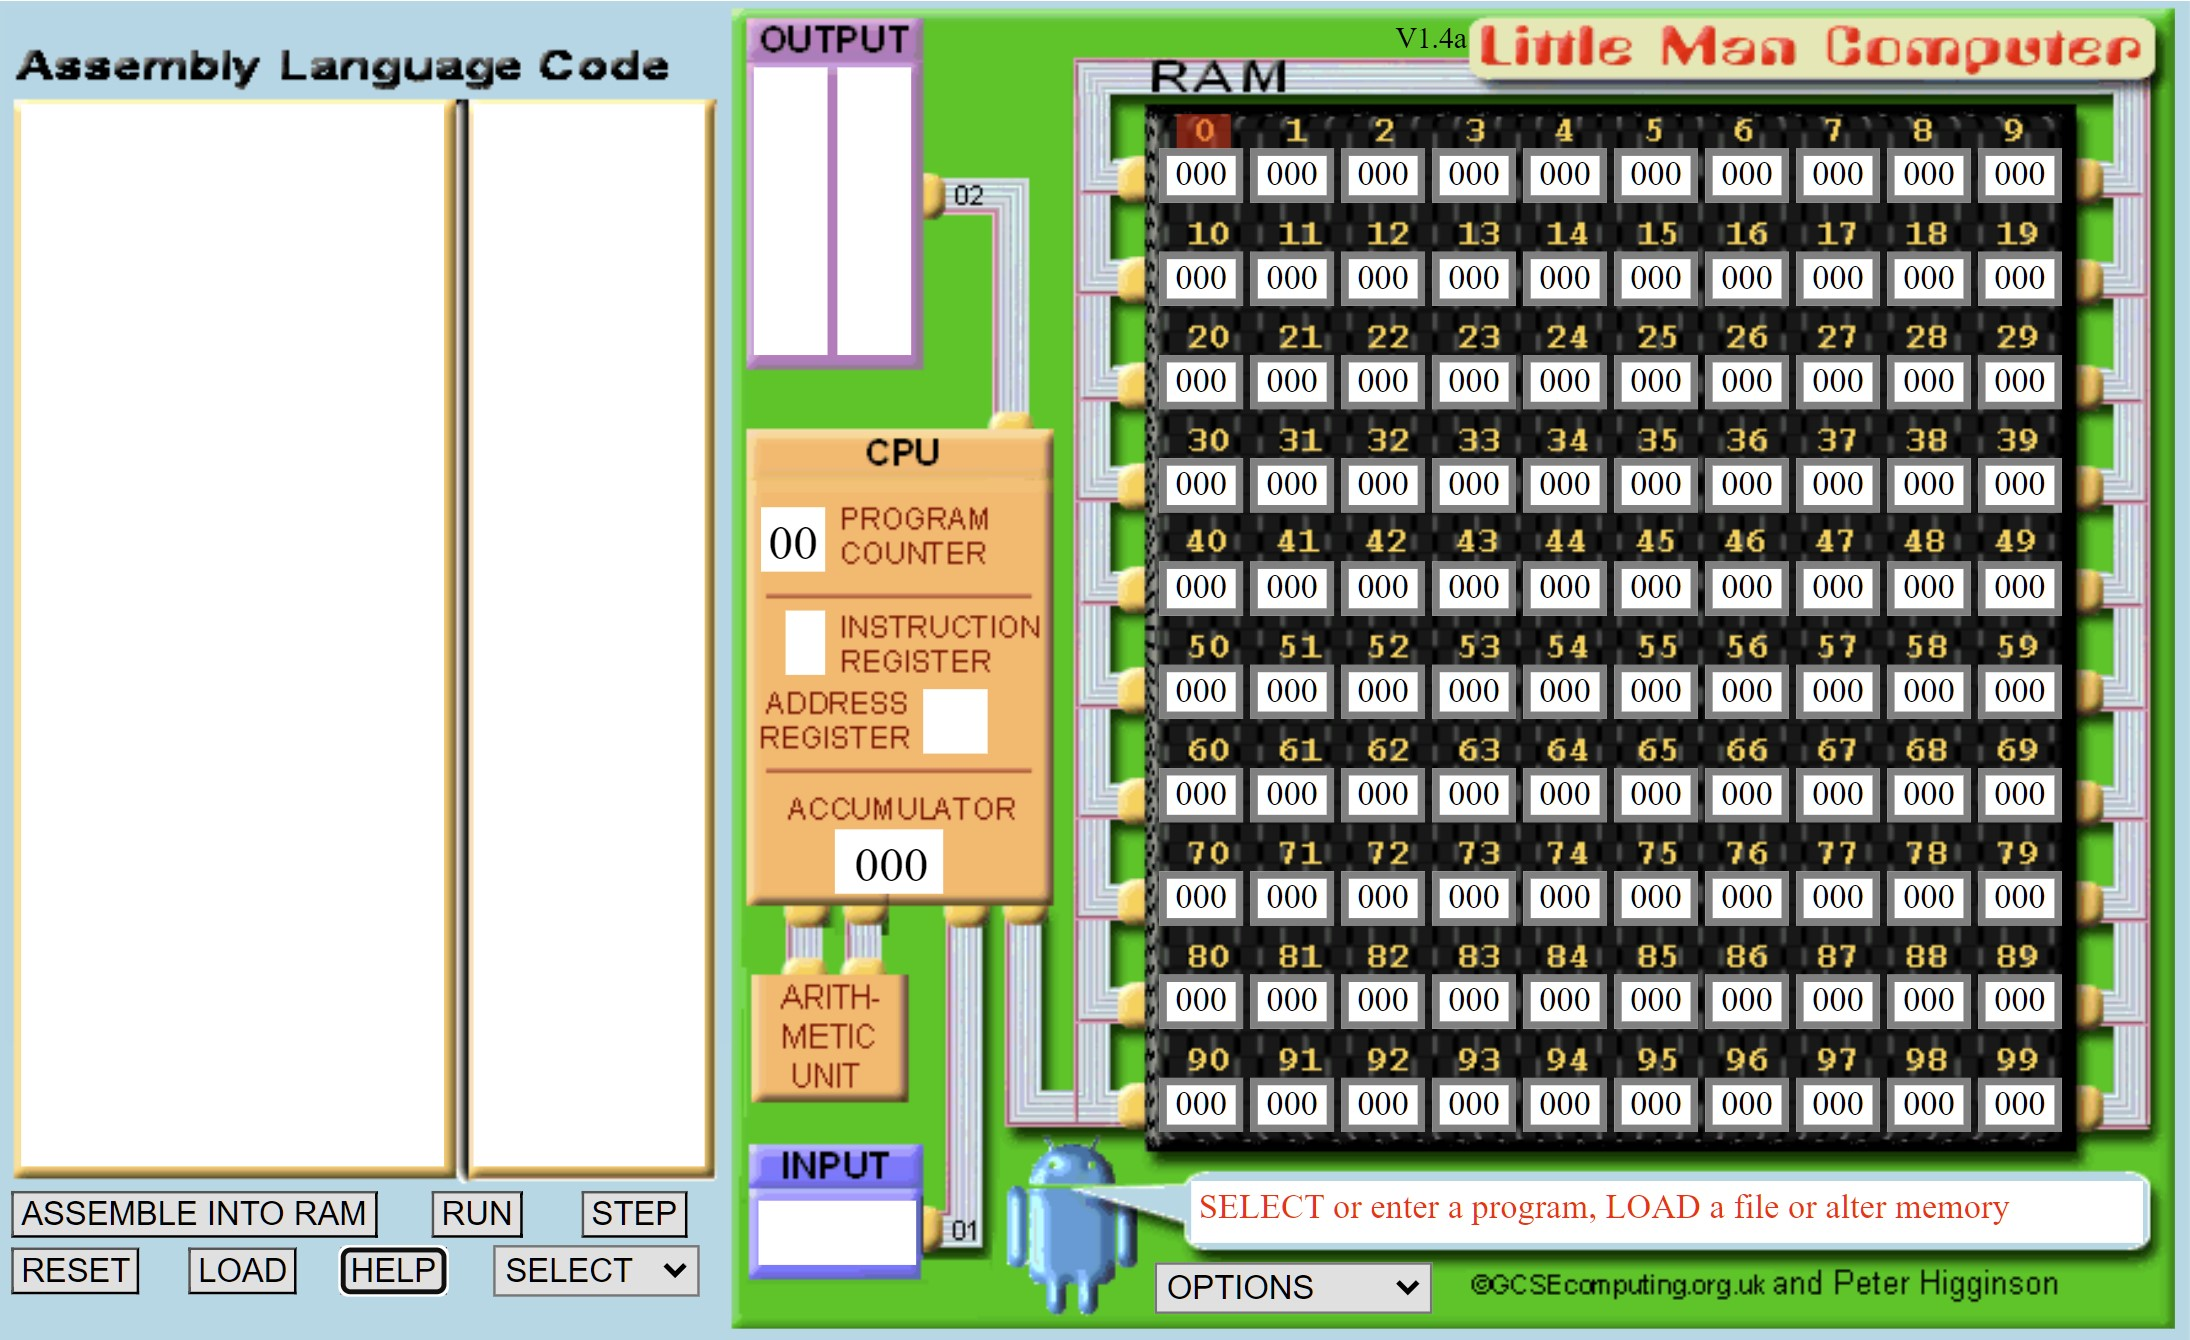
\includegraphics[width=0.75\linewidth]{dissertation/DATA/LMC.jpg}
    \caption{LittleManComputer Simulator by Peter Higginson}
    \label{fig:lmc}
\end{figure}
LittleManComputer \cite{higginson_2014_little} is a instructional model of the computer created in 1965. In 2014, Peter Higginson created a visual simulator \cite{higginson_2014_little} for LMC.

Built purely in JavaScript, it provides a simple interface to visualise the interactions of LMC as instructions manipulate data flowing around the registers and memory.

\begin{table}[h]
\begin{tabular}{|p{0.5\linewidth} | p{0.5\linewidth}|}\hline
\textbf{Pros}                                                     & \textbf{Cons}                             \\\hline
Simple to understand and follow                                   & Not based on RISC-V                       \\\hline
Applicable to all age ranges, younger user will have little issue & Too simplistic for our use                \\\hline
Supports text I/O                                                 & Doesn't operate on registers, only memory \\\hline
\end{tabular}
\end{table}

\subsection{Emulsiv}\label{sec:emulsiv}
\begin{figure}[H]
    \centering
    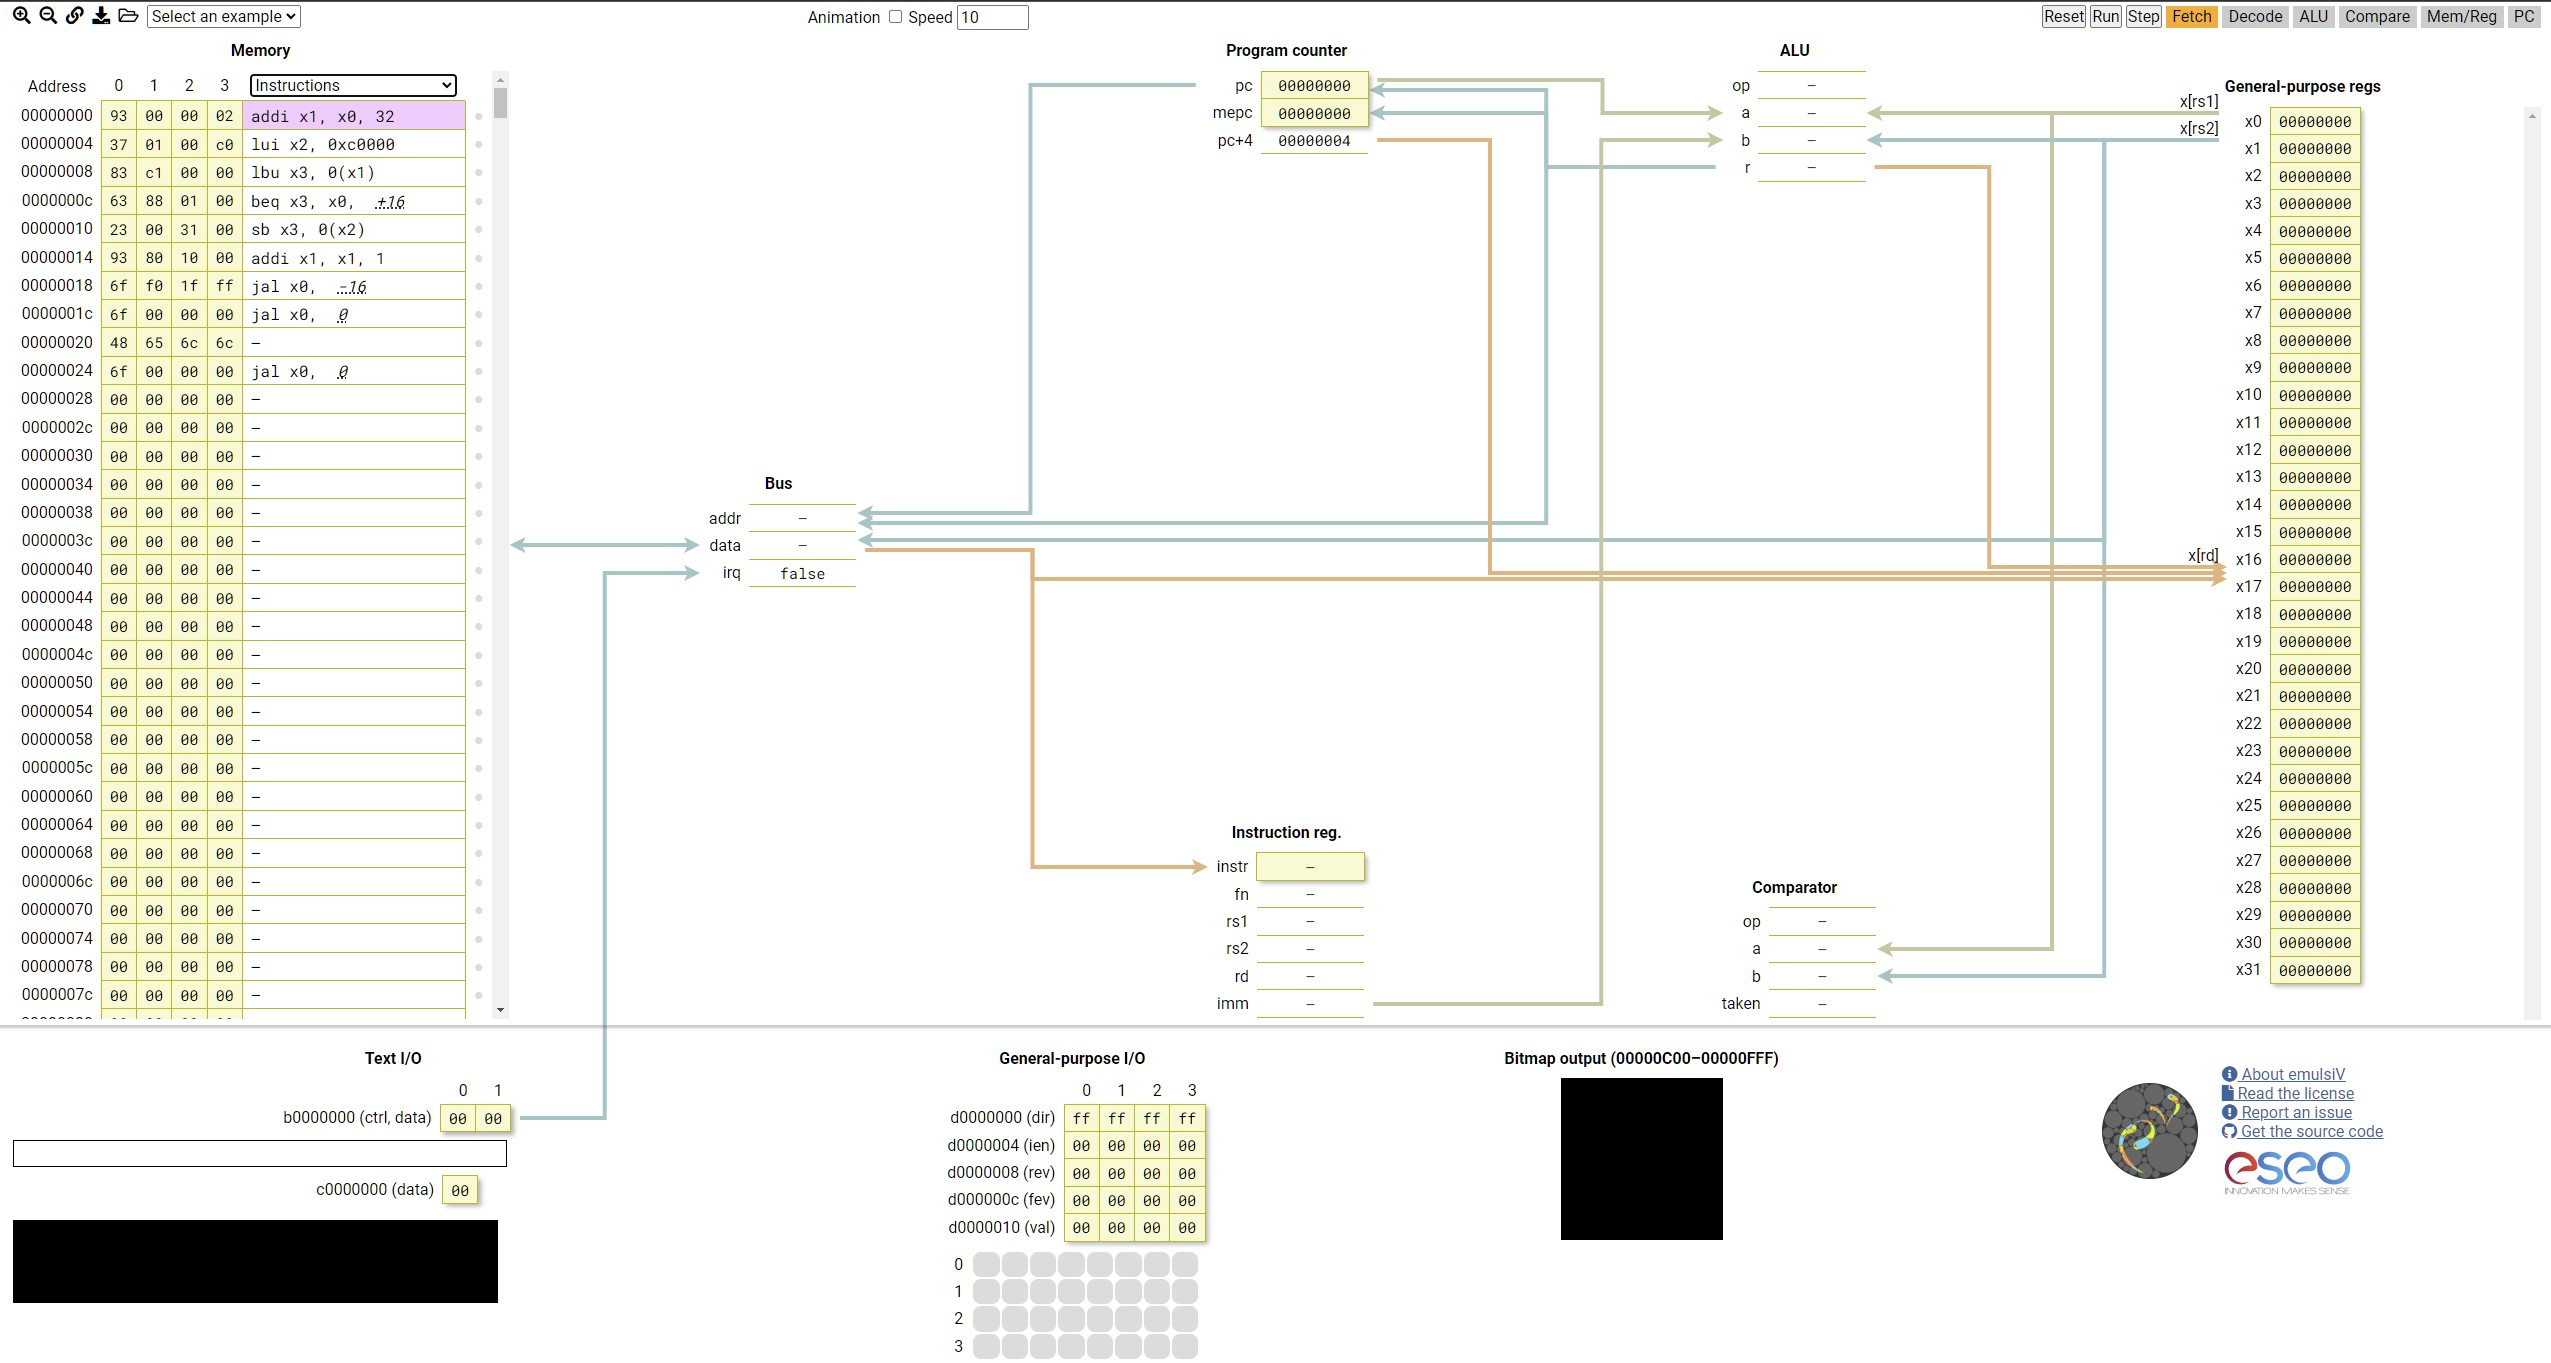
\includegraphics[width=0.85\linewidth]{dissertation/DATA/EMULSIV.jpg}
    \caption{Emulsiv by Guillaume Savaton}
    \label{fig:emulsiv}
\end{figure}
Emulsiv \cite{savaton_2023_eseotechemulsiv} is a web based RISC-V simulator. It was produced by Guillaume Savaton for ESEO (a French Electronic and Engineering School) to help students understand the inner workings of a RISC-V processor. 

\begin{table}[h]
\begin{tabular}{|p{0.5\linewidth} | p{0.5\linewidth}|}
\hline
\textbf{Pros}                                         & \textbf{Cons}                                                                         \\ \hline
Makes use of the complete base 32 bit instruction set & Provides no way to extend with additional instruction sets                            \\ \hline
Provides Text, General Purpose and Bitmap I/O         & Has no central control unit                                                           \\ \hline
Simple design and animations                          & Overall usage is somewhat complex for beginners, and requires thorough reading to use \\ \hline
\end{tabular}
\end{table}

\subsection{Cornell Interpreter}
\begin{figure}[H]
    \centering
    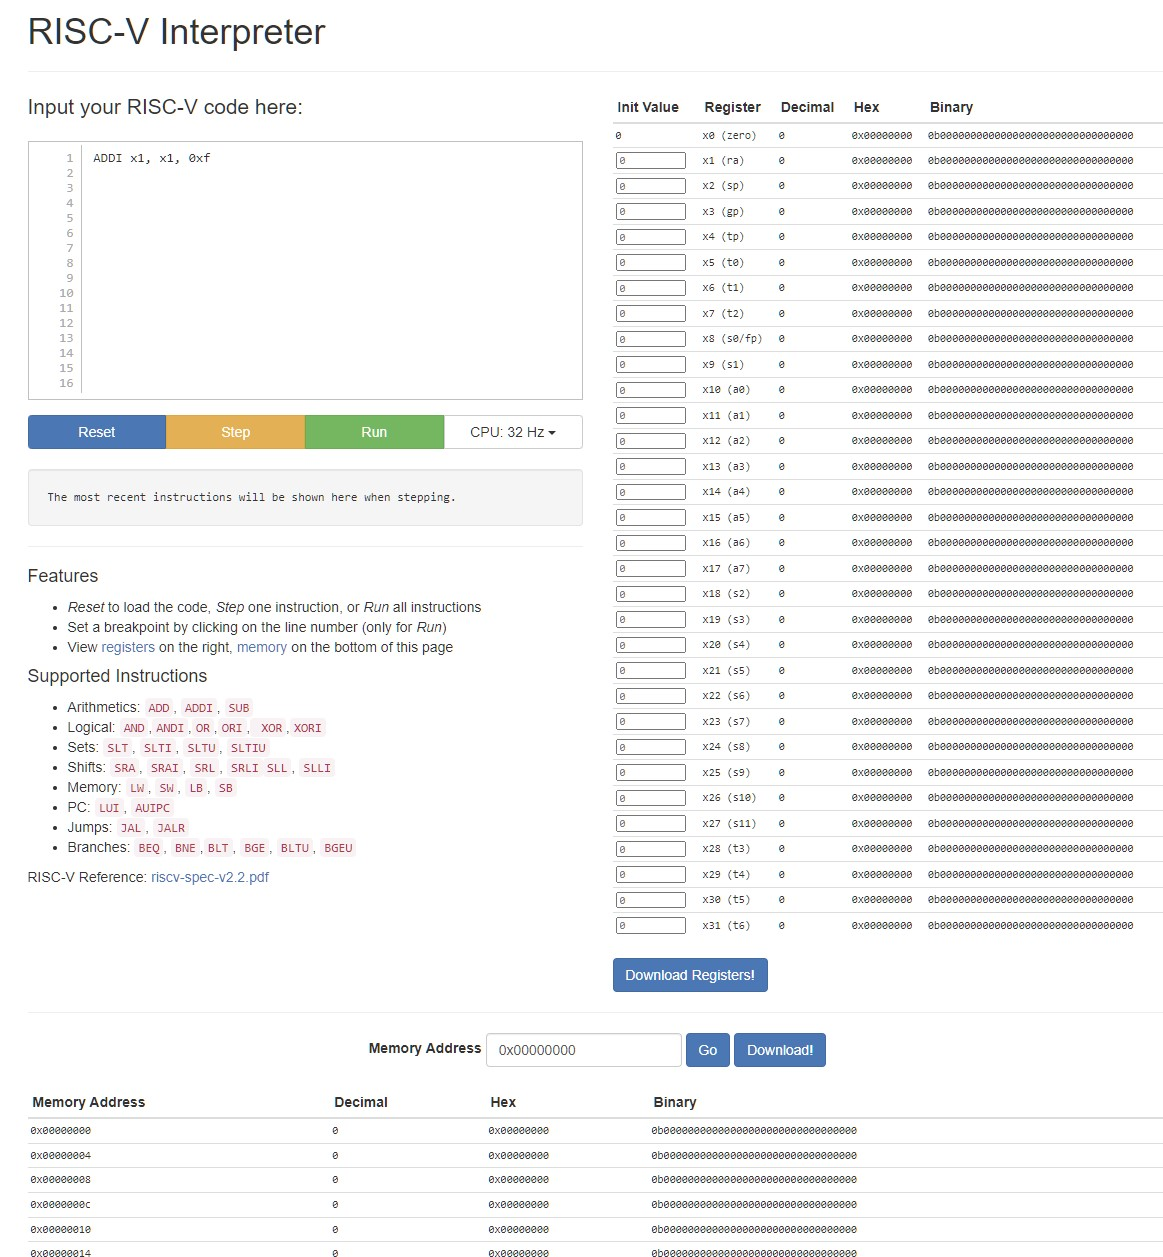
\includegraphics[width=0.75\linewidth]{dissertation/DATA/CORNELL.jpg}
    \caption{Cornell RISC-V Interpreter}
    \label{fig:cornell}
\end{figure}

The Cornell RISC-V Interpreter \cite{cornelluniversity_riscv} was made for the Cornell University CS3410 course. It provides a simple web interface to interpret RISC-V code showing a display of the register and memory changes only, whilst supporting a subset of the base 32 bit instruction set.

\begin{table}[h]
\begin{tabular}{|p{0.5\linewidth} | p{0.5\linewidth}|}
\hline
\textbf{Pros}                                         & \textbf{Cons}                                                                         \\ \hline
Makes use of the complete base 32 bit instruction set & Provides no way to extend with additional instruction sets                            \\ \hline
Provides Text, General Purpose and Bitmap I/O         & Has no central control unit                                                           \\ \hline
Simple design and animations                          & Overall usage is somewhat complex for beginners, and requires thorough reading to use \\ \hline
                                                      &  Very limited overall visualisation options                                                                                      \\ \hline
\end{tabular}
\end{table}

\subsection{rvemu}
\begin{figure}[H]
    \centering
    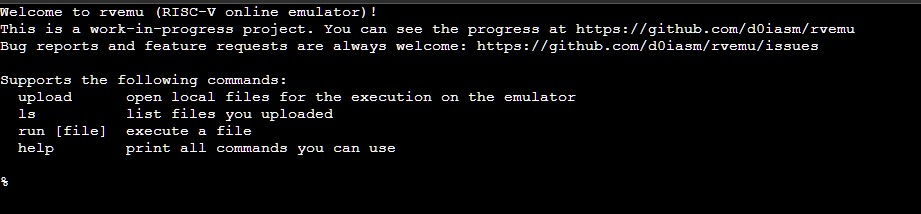
\includegraphics[width=0.85\linewidth]{dissertation/DATA/RVEMU.jpg}
    \caption{rvemu by Asami Doi}
    \label{fig:rvemu}
\end{figure}
rvemu \cite{doi_2021_d0iasmrvemu} is a RISC-V emulator created by Asami Doi in Rust. It provides a CLI interface to load and emulate written RISC-V code. It supports the full 64 bit implementation and many of the 64 bit extensions. However, it provides no visualisation whatsoever other than the end results of a scripts execution.

\begin{table}[H]
\begin{tabular}{|p{0.5\linewidth} | p{0.5\linewidth}|}
\hline
\textbf{Pros}                                                        & \textbf{Cons}                                           \\ \hline
Simple to use                                                        & Doesn't support the full base 32 bit instruction set    \\ \hline
Simple and easy to follow updating of registers and memory           & No way to extend with additional instruction sets       \\ \hline
Allows stepping of instructions, and to simulate at different speeds & No visualisation other than register and memory changes \\ \hline
                                                                     & Very limited overall visualisation                      \\ \hline
\end{tabular}
\end{table}

